\documentclass[twocolumn]{article}
\usepackage[top=1in, bottom=1in, left=1in, right=1in]{geometry}
\usepackage{graphicx}
\begin{document}

\title{Organ Sound Synthesis by Harmonic Interpolation}
\author{Matt Jibson}

\maketitle{}

\begin{abstract}

In this paper I present a method of synthesizing pipe organ sounds by interpolating harmonics of recordings. This method allows unique waves to be generated at all frequencies without the need for sample playback or playback rate manipulation.

\end{abstract}

\section{Introduction}

For those unfamiliar with some of the physics of sound creation, here is a brief primer. A piano and a violin, when playing the same note (i.e., sounding the same pitch), are discernible due to the harmonic structure of the created sound. When a specific note is played, resonance occurs producing a sound at a specific frequency called the base or fundamental frequency. In addition, some to all frequencies that are positive integer multiples of that base frequency are also produced. These frequencies are called the harmonic series. For example, if a note is played with a base frequency of 200Hz, harmonics at 400Hz, 600Hz, etc. are also produced. Some instruments only generate the odd harmonics (e.g., from the base of 200Hz, 400Hz is skipped and 600Hz remains, etc.). The trend of these harmonics is to decrease in power as distance from the base frequency increases. Other frequencies which are not positive integer multiples are also produced with, in general, much lower power, but with a similar decreasing trend. Hence, these differences in harmonic structure produced aural (heard) differences between instruments.

Pipe organs are unique wind instruments in that each sound is generated by its own pipe. This is in contrast with other wind instruments where the effective length of a single pipe is changed with valves (e.g., trumpet), holes that are covered (e.g., clarinet), or a slide (e.g., trombone). This, by nature, creates variations in the harmonics of each pipe (and thus over the entire range) because of slight fabrication differences or purposeful voicing differences by the builder. In contrast, other wind instruments, which are based on a single piece of metal or wood, have a similar harmonic structure over their entire range.

Current sound generation techniques for organs generally involve some combination of (1) playback of pre-recorded samples (2) sampling frequency manipulation to adjust perceived pitch, and (3) wave tables from which specific pitches can be generated. The first method, which requires organ tuning, recording, and editing of samples sets is expensive time consuming, data intensive, and limits playback to only recorded pitches. The second method, when combined with the first, allows any pitch to be produced, but at exact harmonic structure as the original sample. The third method, based from recordings, shares properties of both, in that specific pitches can be generated, but if not specifically in the table, will have exact harmonic structure as other outputs. Hence, all no current method is cheap, easily available and accurate to organ acoustics.

In order to create a method that meets those requirements, it must be (1) produceable cheaply and (2) model a harmonic structure across an entire range. In order to meet the first requirement, recordings will be limited in number and quality: only one note per octave, which need not be in tune. To meet the second requirement, a set of continuous functions must be produced which will be able to generate unique outputs at any frequency.

\section{Method}

\subsection{Recording Analysis}

After recordings of the chosen notes are made and edited to include only the primary pipe speech (i.e., after the initial attack and before the final release of the note, Figure \ref{time}), each recording is processed through a power spectral density (PSD) function (Figure \ref{psd}). A PSD function determines the power distribution of a signal in the frequency domain. This allows us to see the power of the signal at discrete frequencies. The $N$ (an arbitrary number chosen by the user) largest peaks in each distribution are found by searching for three consecutive points where the middle point has greater value than both surrounding points (Figure \ref{peaks}). The percentage power contribution of each peak is found by dividing the power of the peak by the total power of the distribution. Finally, the expected base frequency is recorded as the closest frequency to it that is also one of the $N$ peaks. We cannot use an exact base frequency because the PSD function produces a list of discrete frequencies. Furthermore, the number of peaks chosen so that there is a close match (within 2Hz, generally). This is generally not an issue as the base frequency is almost always one of the first two peaks.

\begin{figure}
\centering
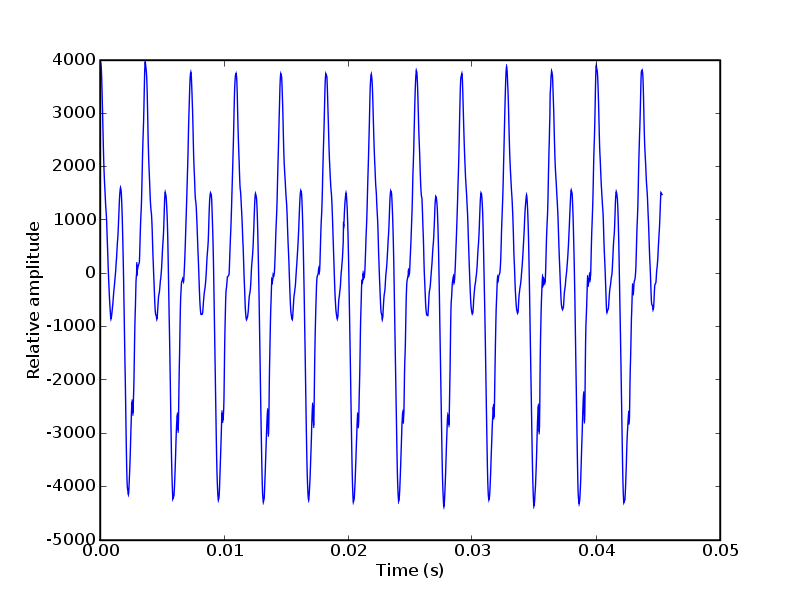
\includegraphics[width=\linewidth]{figures/time.png}
\caption{Excerpt of a recorded wave, shown in the time domain.}
\label{time}
\end{figure}

\begin{figure}
\centering
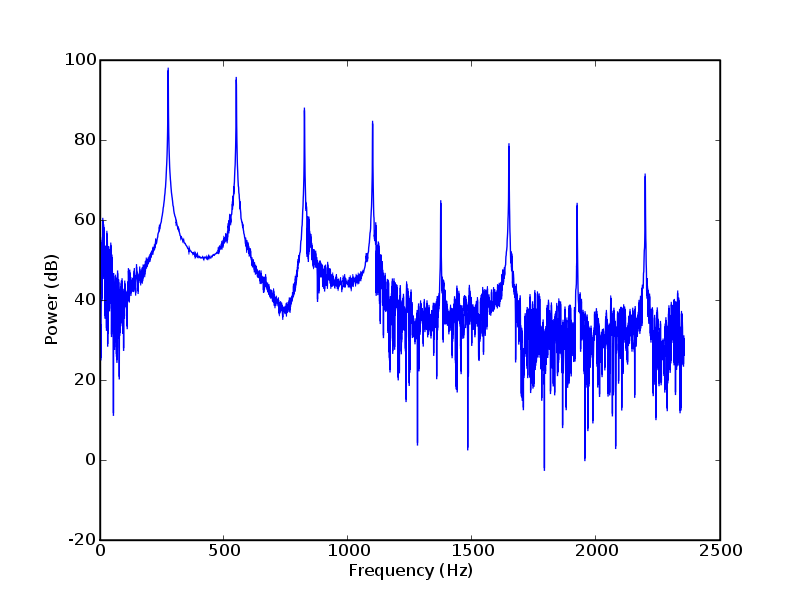
\includegraphics[width=\linewidth]{figures/psd.png}
\caption{Excerpt of the PSD of a recorded wave, shown in the frequency domain.}
\label{psd}
\end{figure}

\begin{figure}
\centering
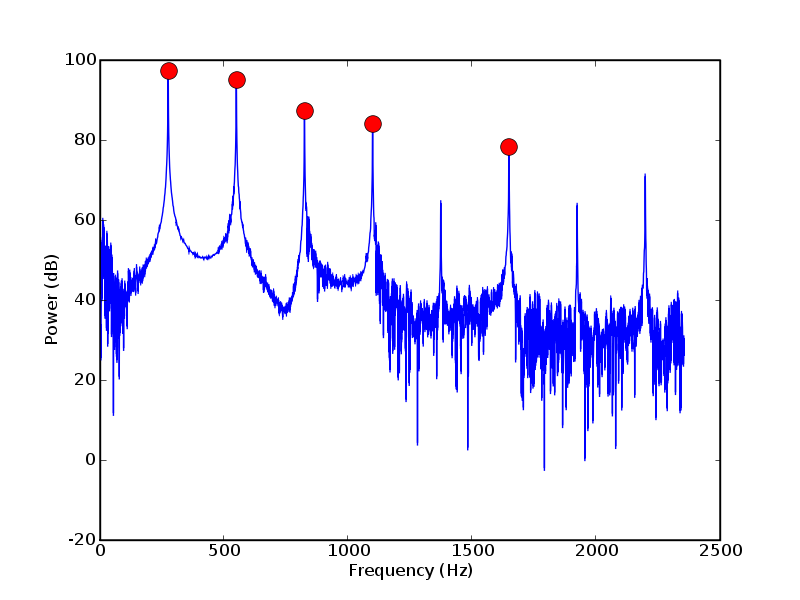
\includegraphics[width=\linewidth]{figures/peaks.png}
\caption{Excerpt of the PSD of a recorded wave, shown in the frequency domain. The first five peaks are marked with red circles.}
\label{peaks}
\end{figure}

At this point processing on individual recordings is complete and they may be processed as a set. The first peak power contribution of each recording is taken, along with that recording's base frequency. A least squares polynomial fit algorithm is applied with $x$ values (sample points) as base frequencies, and $y$ values (values to fit) as the peak power contribution corresponding to that base frequency. A degree of 3 tends to produce good results. This is repeated for all of the other $N$ peaks (e.g., the polynomial fit algorithm is applied to all of the second, third, etc. peak power contributions up to $N$). These algorithms generate $a$s, $b$s, and $c$s for the polynomial $a x^2 + b x + c = y$, where $x$ is the desired frequency and $y$ is the resultant power contribution for each of the first $N$ power contributions, which gives us continuous functions from which to generate individual (and likely unique) waves at any frequency harmonic structures.

\subsection{Sound Synthesis}

To synthesize a desired sound at base frequency $F$Hz, find the frequencies of the $N$ peaks of the recording with the closest base frequency to $F$. (Alternatively, other search methods can be used. For example, if there is such a frequency, find the recording with the closest base frequency to $F$ that is not greater than $F$.) Generate sinusoids at these frequencies at desired lengths and sampling frequencies. Apply $F$ as $x$, taking output as $y$ to the polynomial described above associated with each peak's power contribution. Scale (e.g., multiply) each value from the generated waves by $y$. Add the waves together (i.e., add the first, second, third, etc. value of each wave together), producing the output wave.

\section{Results}

Results by listening test are acceptable. The produced sound is clearly of correct pitch and timbre. It is also, however, clearly computer generated. Furthermore, when going beyond the range of the lowest and highest recorded sounds, the generated sounds can get wildly inaccurate, with the percentage contribution multipliers quickly blowing up, yielding meaningless results. Thus, generated sounds should be confined to the interval between the lowest and highest recorded notes, or within a small margin thereof.

As a result of using the closest recorded note to the desired frequency as the basis for the harmonic structure, there are very noticeable changes when listening to a full range sweep of produced noises (i.e., a generated tone corresponding to each note on an organ). This occurs when the closest recorded note switches to another recorded note. The change in harmonic structure is noticeable since it is so abrupt and unnatural.

Regarding a computer back-end, this method meets our requirements of real-time speed. Generating sinusoids at a certain sampling frequency (say, 48kHz) for $N$ peaks (say, 50) is about 2.4 million samples per second. A sample involves a sinusoid operation, two multiply operations, plus some trivial operations that have no significant performance effect. Modern computers run in the billions of operations per second range, or around two to four orders of magnitude faster than required to process real-time requests of a naive implementation. There is thus computational availability for multiple notes. With an optimized, cached, or preprocessed data, this availability can increase further.

Processing speed of this algorithm is on the order of seconds-per-recording. The PSD function, which involves many Fast Fourier Transforms, is the most expensive computationally. However, we do not care much about this time since it need only be done once, and typically before use where the time constraints are lenient.

\section{Discussion and Further Work}

As touched on above, there are some boundaries between notes on a full range where the harmonic structure noticeably changes from one recorded note's structure to another's. It is not possible to simply apply a polynomial fitting algorithm to the harmonics as was done in the power contribution case. Let us assume, for example, a set consisting of two recordings, one octave apart. Both recording have as their most powerful frequency their base frequency. The lower recording has as its second most powerful frequency twice the base frequency, as we would expect from a classic harmonic series. The higher recording, however, has as its second most powerful frequency triple the base frequency. We cannot, of a certainty, interpolate so that each step in between is a $1/12^\mathrm{th}$ increase (i.e., the first note above the lowest recording's second most powerful frequency is 1.083 of the base frequency, the second note 1.166 of the base frequency, etc.). This approach produces results that do not sound the correct pitch, which is expected, since they do not follow the harmonic series at all. In general, the harmonics above the base are taken from a list. They tend to be integer multiples above (or below) the base frequency. Thus, we can look at the solution as something that will be somewhat discretized, with choices taken from a list with a certain probability to each, perhaps Gaussian distributed. Other algorithms involving optimization and genetic algorithms may suggest other models. These algorithms and models, when applied to data from a recording set over a full range of notes, may yield methods to generate individual harmonic structure for all frequencies.

Of interest to sound engineers and others interested in vocoders is the possibility of applying this method on a recording set not consisting of all one instrument. For example, a recording set of a bass drum, oboe, and voice may produce unique results with varying components of each at all ranges. This application, however, is not worth while until the harmonic structure is a function of frequency, as discussed in the proceeding paragraph.

This method does not model many parts pipe speech: (1) the beginning of pipe speech, called chiff, is an important part of all pipe organs that is specifically modified (not removed) by the builder during installation; (2) the end of pipe speech, which is of less importance; (3) sibilance, the sound of air moving over a pipe mouth during nominal speech. Without these it is clear that the produced sound does not come from a genuine pipe. The above method works well on sounds that have a few significant frequencies making up much of the sound. These three parts of pipe speech have no such property, and so are perhaps modeled better in the time domain, instead of the frequency domain.

\section{Conclusion}

I have presented a novel approach to sound synthesis meeting requirements that current implementations cannot. While in an introductory phase, this method has shown promising results and proof-of-concept implementation. Further work is warranted.

\end{document}
